% This work is licensed under the Creative Commons Attribution-NonCommercial 4.0 International License.
% To view a copy of this license, visit http://creativecommons.org/licenses/by-nc/4.0/
% or send a letter to Creative Commons, PO Box 1866, Mountain View, CA 94042, USA.

% !TEX TS-program = xelatex

\documentclass[../Main/notes.tex]{subfiles}

\setcounter{chapter}{6}
\begin{document}

\chapter{Open-shell species}



So far we have only discussed the electronic structure of closed-shell molecules and glossed over open shell species.
In this chapter we will look at how Hartree--Fock and Kohn--Sham theory can be applied to open-shells.
We will first classify open-shell species and then discuss the theoretical formalisms available to do computations.
Lastly, we will discuss classes of open-shell systems that cannot be computed accurately with Hartree--Fock and Kohn--Sham theory.

\section{What do we mean when we talk about open-shell species?}

\emph{Closed-shell atoms or molecules} contain an even number of electrons and are well described by a single electron configuration in which orbitals are either doubly occupied or empty.
Some examples are the Ne atom, the water molecule, most stable organic molecules, etc.

\emph{Open-shell species} are instead characterized by having unpaired electrons and have radical character.
Since unpaired electrons can have alpha or beta spin, there are different types of open-shells.
If all the unpaired electrons have the same spin (say all alpha), then we talk of a high-spin open shells.
High-spin open shell systems have nonzero spin which makes the paramagnetic.
An example of this is the OH$^\cdot$ radical (doublet) with one unpaired electron, or oxygen (\ce{O2}) and methylene (\ce{CH2}), which both have a ground state with two unpaired electrons (a triplet diradical).
Open-shell character can also arise if electron pairs are broken preserving the spin of each electron (one alpha and one beta electron per pair), leading to low-spin states.
For example, the ozone molecule (\ce{O3}) or \textit{p}-benzyne are considered to be species with pronounced open-shell character because they have partial diradical character (but no net spin).
Many transition state compounds also display low-spin open shell states.


\mfigure{
\centering{
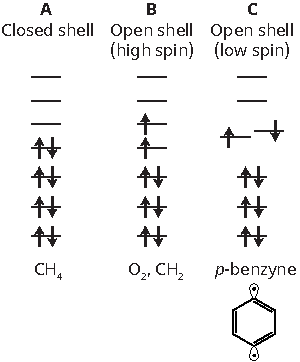
\includegraphics[width=1.75in]{img/open-shells.pdf}
}
\captionof{figure}{Illustration of the main electron configuration for closed-shell molecules (\textbf{A}), high-spin open shells (\textbf{B}), and low-spin open shells (\textbf{C}). For the low-spin open shell case (\textbf{C}) only one Slater determinant is shown.}
\label{fig:open-shells:open-shells}
}

\section{Spin, multiplicity, and all of that}

To understand how computation on open-shell species work, it is necessary to grasp some elementary facts about the quantum mechanics of spin.
Spin is a vector quantity like angular momentum, so we can associate three Cartesian components to it, to which correspond three operators $\hat{S}_x$, $\hat{S}_y$, and $\hat{S}_z$.
If we want to describe the spin of an atom or a molecule, quantum mechanics allows us to specify two quantities:
\begin{enumerate}
\item The square of the total spin, to which corresponds the operator $\hat{S}^2 = \hat{S}_x^2 + \hat{S}_y^2 + \hat{S}_z^2$.
This operator measures the magnitude of spin (like you would measure the length of a vector).
For electrons, the eigenvalue corresponding to this operator is $s(s + 1)$ (in atomic units), where $s$ is the \emph{total spin quantum number}.
For an electron $s = 1/2$ and the total spin squared is equal to $3/4$.

\item One consequence of the rules of spin in quantum mechanics, is that eigenstates cannot be characterized by knowing all the components of spin.
We can only pick one component, and typically we choose the projection of spin onto the $z$ axis. This quantity corresponds to the operator $\hat{S}_z$.
The eigenvalues of this operator are controlled by the quantum number $m_s$ which ranges from $-s$ to $+s$ in increments of one.
\end{enumerate}
\emph{In the absence of a magnetic field},\mnote{Ignoring relativistic effects.} a level with total spin quantum number $s$ has $2s + 1$ degenerate states. The number of degenerate states for a given spin multiplet is called the \emph{multiplicity}.
For example, a single electron has $s = 1/2$, which means that it can have two allowed values of $m_s$
\begin{equation}
m_s = \begin{cases}
+1/2 & \text{alpha spin} \\
-1/2 & \text{beta spin}
\end{cases}
\end{equation}
We say that the \emph{multiplicity of this state is two}, and call it a doublet.\mnote{Singlet = one state, doublet = two states, triplet = three states, quartet = four states, quintet = five states, sextet = six states, \ldots}
The same result applies to molecules with one electron like \ce{H2+}.

When there are more than one electron the spin of a state is still characterized by two quantum numbers that we write as capitals $S$ and $M_S$.
The total spin squared quantum number can be any of
\begin{equation}
S = 0, 1/2, 1, 3/2, \ldots
\end{equation}
and the z-projection of spin quantum number can take any of the values
\begin{equation}
M_S = -S, -S + 1, -S + 2, \ldots, S-2, S -1, S
\end{equation}
the \emph{multiplicity} of a state, defined as the number of degenerate spin states corresponding to one value of quantum number $S$ is given by
\begin{iequation}
\text{multiplicity} = 2S + 1
\end{iequation}

The values of $S$ and $M_S$ depend on the electron state.
The total projection of spin on the z axis is computed as the difference between the number of alpha and beta electrons divided by two
\begin{iequation}
M_S = \frac{1}{2} \left(N_\alpha - N_\beta \right)
\end{iequation}
For example, in the case of a high-spin open-shell species like \ce{CH2}, with five alpha and three beta electrons, the value of $M_S = (5 - 3) / 2 = 1$.

\emph{For the high-spin case} when  the unpaired electrons are all alpha or all beta, $M_S$ and $S$ are related by
\begin{equation}
S = |M_S|
\end{equation}
The case of low-spin states is a bit more involved, and we will not consider it here.

\begin{example}[The nitrogen atom]
The nitrogen atom has an electron configuration 1s$^2$ 2s$^2$ 2p$^3$.
According to Hund's rule, the ground state of N is a high-spin state with three alpha electrons in the 2p orbitals. Consequently, the N atom has 5 alpha electrons and 2 beta electrons.
The $M_S$ value for this state is $(5 - 2)/2 = 3/2$.
This state has the highest value of $M_S$ compatible with the  electron configuration 1s$^2$ 2s$^2$ 2p$^3$ (because all the unpaired electrons are alpha), therefore it must corresponds to a component of a multiplet with $S = 3/2$.\mnote{If this was not the case we would be able to construct a state with a higher value of $M_S$, say $5/2$.
But to get this value of $M_S$ we would have to have six alpha electrons and 1 beta electron. This state is incompatible with the 1s$^2$ 2s$^2$ 2p$^3$ electron configuration. Try it out.}
The multiplicity of the ground state of the N atom is then $2 \times 3/2 + 1 = 4$, and the state is a \emph{quartet}. So to run a computation on the N atom you need to use the following input geometry (in xyz coordinates)
\begin{verbatim}
0 4
N 0.0 0.0 0.0 
\end{verbatim}
\end{example}

\begin{example}[The \ce{NO-} molecule]
The \ce{NO-} molecule is isoelectronic with the oxygen molecule and contains a total of 16 electrons.
The MOs of \ce{NO-} are shown below together with the electron occupation (the core 1s-like orbitals are not shown here)
\begin{center}
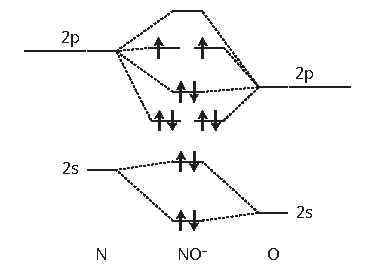
\includegraphics[width=2.5in]{img/no-.pdf}
\end{center}
Since the last two electrons fill in a pair of degenerate $\pi$ orbitals, electron repulsion favors a high spin open shell configuration with electrons in different orbitals.
This high spin state of  \ce{NO-} has 9 alpha electron and 7 beta electrons, which corresponds to a $M_S$ value equal to $(9 - 7)/2 = 1$.
Since for this high spin state $S = 1$, the multiplicity is three and the state is a triplet.
To run a computation on the \ce{NO-} molecule you need to use the following input geometry (in Z-matrix coordinates)
\begin{verbatim}
-1 3
N
O 1 <NO distance>
\end{verbatim}
\end{example}

\section{How do quantum chemistry codes handle (high-spin) open-shell HF and DFT computations?}

\emph{What is important to realize, is that for HF and DFT computations, most quantum chemistry codes assume that we are dealing with the high-spin open-shell case}.
When you specify the input geometry you are also providing the charge and multiplicity of your molecule.
The charge is the sum of the positive nuclear charges ($Z_i$) minus the number of alpha/beta electrons ($N_\alpha$, $N_\beta$)
\begin{iequation}
\text{charge} = Q = \sum_i^\text{nuclei} Z_i  - (N_\alpha + N_\beta)
\end{iequation}
The multiplicity is instead $2S + 1$, and since for a high-spin open-shell species $S = |M_S|$, we have that
\begin{iequation}
\text{multiplicity} = 2 M_S + 1= \left(N_\alpha - N_\beta \right) + 1
\end{iequation}
From these two equations, a quantum chemistry codes computes the number of alpha and beta electrons.

In Hartree--Fock theory, there are two ways to perform computations on open shell systems that differ in the way the alpha and beta orbitals are treated.
In the \emph{restricted open-shell} (RO) formalism, alpha and beta orbitals occupy orbitals that have the same spatial function. Therefore, the RO formalism enforces the condition
\begin{equation}
\phi_{i\alpha}(\mathbf{r}) = \phi_{i\beta}(\mathbf{r})
\end{equation}
for all orbitals.
One of the advantages of the ROHF approach is that the resulting Slater determinant is an eigenfunction of spin.
This means that it has an average value of $S$ that is integer or a half-integer number.

In an \emph{unrestricted} (U) formalism, the alpha and beta orbitals have different spatial part
\begin{equation}
\phi_{i\alpha}(\mathbf{r}) \neq \phi_{i\beta}(\mathbf{r})
\end{equation}
Note that \emph{for a single electron}, these two approaches give the same energy.
With more than one electron these two methods give different results.
The UHF energy is usually lower than or equal than the ROHF energy.
This is consequence of \emph{spin contamination} by electronic states with spin higher that the value one would expect ($S = |M_S|$).
%In a spin contaminated solution.
%Why does spin contamination happen?



\mfigure{
\centering{
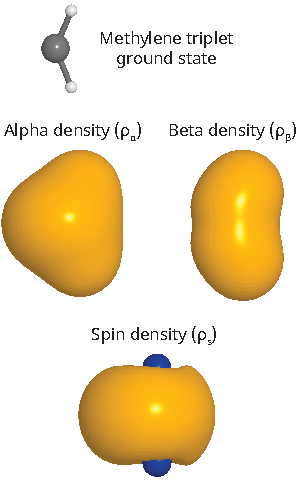
\includegraphics[width=1.75in]{img/methylene.pdf}
}
\captionof{figure}{Alpha, beta, and spin densities of methylene (\ce{CH2}). Yellow (blue) surfaces indicate positive (negative) spin density.}
\label{fig:open-shells:methylene}
}

In DFT, one may use either the RO or the U formalism. However, only the unrestricted Kohn--Sham approach is formally justified.\mnote{Some implementations of DFT include the ROKS formalism. However, you should never use it.}
Since the Kohn--Sham approach should yield the exact density of alpha and beta electrons ($\rho_\alpha$ and $\rho_\beta$), one can obtain the exact \emph{spin density} ($\rho_s$) that measures the excess or lack of alpha electrons in space.
The spin density is defined as
\begin{equation}
\rho_s(\mathbf{r}) = \rho_\alpha(\mathbf{r}) - \rho_\beta(\mathbf{r})
\end{equation}
and for an open-shell species can be positive or negative (it is identically zero for closed-shell molecules).
In a ROKS approach the spin density is constrained to be positive ($\rho_s \geq 0$), while the UKS approach may yield both positive and negative values of $\rho_s$.
In general, open-shell molecules will display regions where the spin density is positive and negative, and therefore, only the UKS formalism can correctly describe open shells.
An example is given by the triplet state of the methylene, shown in Fig.~\ref{fig:open-shells:methylene}. In this molecule the spin density is negative on the carbon atom (indicating an excess of alpha electrons, in yellow), while the hydrogen atom carry an excess of beta electrons (negative spin density, in blue).
This is perhaps surprising because one would expect that the extra two alpha electrons would be distributed all over the molecular frame.

Even the ROHF formalism cannot describe molecules with negative spin density, but as we will see later, there are methods to systematically improve the wave function starting from ROHF.
Therefore, ROHF remains is a valid approach for computing high-spin open shells.

\section{Low-spin open shells, bond breaking processes, and other problems that require a multideterminantal description}

\mfigure{
\centering{
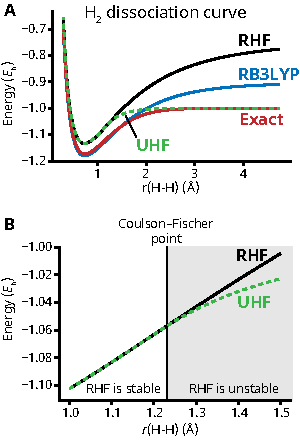
\includegraphics[width=2.00in]{img/h2.pdf}
}
\captionof{figure}{Dissociation curve of \ce{H2} computed with the aug-cc-pVTZ basis set and various computational methods. (\textbf{A}) Comparison of restricted Hartree--Fock (RHF), restricted Kohn--Sham using the B3LYP functional (RB3LYP), full configuration interaction (Exact), and unrestricted Hartree--Fock (UHF).
(\textbf{B}) detail of the transition from a stable to an unstable RHF solution at the Coulson--Fischer point.}
\label{fig:open-shells:h2}
}

As we have seen, high-spin open shell molecules can be treated both with HF and DFT (as well as correlated methods).
There are cases, like low-spin open shells and bond breaking processes, that cannot be studied with these methods.
These systems are associated with a type of correlation called \emph{static, non-dynamical, or strong}, which cannot be accurately described by a single Slater determinant.
Static correlation is also problematic for Kohn--Sham DFT using approximate functionals.

The simplest example of static correlation is homolytic bond breaking in  diatomics.
The top panel of Fig.~\ref{fig:open-shells:h2} shows the dissociation curve of \ce{H2} computed with restricted HF, restricted Kohn--Sham (using the B3LYP functional), and the exact solution (computed with the full configuration interaction method, FCI).
Both the RHF and RB3LYP results lead to dissociation energies that are significantly higher than the exact values.
Specifically, the RHF dissociation energy is almost twice as large as the exact value, and while the exact dissociation curve is already flat for bond lengths greater than 3 \AA{}, the HF curve keeps rising and never flattens.
Why is the RHF (and RB3LYP) dissociation curve incorrect?
One can formally show that the single Slater determinant approximation used in HF leads \ce{H2} to dissociate to the wrong states.
At infinite distance, the HF solution converges to an electronic state that is a 50/50 combination of two \emph{covalent} terms plus two spurious \emph{ionic} terms
\begin{equation}
\begin{split}
\text{restricted Hartree--Fock} & = \quad \underbrace{25\% \; (\ce{H}^{\uparrow} + \ce{H}^{\downarrow}) + 25\% \; (\ce{H}^{\downarrow} + \ce{H}^{\uparrow})}_{\text{covalent configuration}} \\
& + \quad 
\underbrace{25\% \; (\ce{H+} + \ce{H-}) + 25\% \; (\ce{H-} + \ce{H+})}_{\text{ionic configuration}}
\end{split}
\end{equation}
This solution found by HF is incorrect, because the ionic configuration should not contribute to the wave function when the two hydrogens are at infinite distance.
The ionic configuration is responsible for the higher dissociation energy due to the Coulomb interaction of the oppositely charged ions.
Because this is a long-range interaction, it affects the shape of the potential at large distances causing the curve to not flatten out.

\emph{In the exact solution} the weights of the covalent and ionic configurations \emph{are allowed to change}.
You can think of the exact solution as being a superposition of the covalent and ionic configurations, but with a variable amount of those two terms. At  large \ce{H-H} distances the correct description of \ce{H2} includes only the covalent configuration.
In principle, Kohn--Sham theory should be able applicable to compute the \ce{H2} dissociation curve. However, current approximate functionals are not designed to treat static correlation.\mnote{Recently, approximate density functionals for static correlation have been proposed. These are not widely available.}

If one applies unrestricted HF to the \ce{H2} molecule one obtains the green curve in Fig.~\ref{fig:open-shells:h2} \textbf{A}.
For small \ce{H-H} distances, the RHF and UHF curves are identical.
However, at about 1.23 \AA{} the two curves start to become different.
We call this the \emph{Coulson--Fischer point}.\mnote{When you run a UHF computation, you are not guaranteed to find this lower-energy UHF solution. Calculations must use no symmetry and it might be necessary to do a  stability analysis to guide the SCF procedure to find the lower energy solution.}
Past the Coulson--Fischer point, the UHF energy is lower and it goes to the correct energy limit (about -1 \Eh) in the dissociation limit.
This suggests that one may use UHF to study cases where static correlation is important.
Why does UHF predict the correct energy in the dissociation limit?
An analysis of the UHF orbitals shows that for large \ce{H-H} distances the wave function is composed by a single term in which an electron with alpha spin is localized on one atom and an electron with beta spin is localized on the opposite atom 
\begin{equation}
\text{unrestricted Hartree--Fock} = \quad \underbrace{100\% \; (\ce{H}^{\uparrow} + \ce{H}^{\downarrow}) }_{\text{covalent term}}
\end{equation}
This is called a \emph{symmetry-broken} solution and technically it is not a good wave function because there is only one of the two covalent configurations (the one missing has the electron spins flipped).
Once can show that the symmetry-broken is a combination of a singlet ($S = 0$) and a triplet ($S = 1$) solution.
Indeed, the average value of the total spin operator $S(S+1)$ for the broken-symmetry solution is 1, a value that is in between that of a singlet state (0) and a triplet state (2).

Although unrestricted HF and DFT are often used to treat low-spin open shells, \emph{a proper treatment of these systems requires  multiconfigurational self-consistent theory} (MCSCF).
In MCSCF, the wave function is approximated by a liner combination of Slater determinants $\Phi_{I}$ multiplied by coefficients $C_I$
\begin{equation}
\Psi_{\text{MCSCF}} = \sum_I C_I \Phi_{I}
\end{equation}
In MCSCF, both the orbitals used to construct the determinants $\Phi_{I}$ and the $C_I$ coefficients are variables optimized to find the minimum   energy solution.
\emph{A particularly popular form of MCSCF is the complete-active-space SCF method} (CASSCF). This is the starting point for many methods that can be applied to bond breaking processes, open-shell transition metal compounds, and electronically excited states.
\end{document}
